\chapter{Introduction}

\section{Motivation}
In recent years, English has been more commonly the preferred language of communications in many setting. The assessment of spoken English has therefore become increasingly important, especially in the context of education and employment opportunities. Traditionally, human examiners have been used to evaluate spoken English, but this approach is time-consuming and subjective. As a result, automated systems for spoken language assessment has been developed to assist the examinations.

Candidates taking English speaking exams are from a vastly different background, with different age, gender, accent, and more. As such, it is important to ensure the grading process are unbiased. This means the process should evaluate speech samples solely based on performance-related factors, such as vocabulary richness and fluency, without being influenced by irrelevant attributes like gender, age and first language. It is important to ensure that the grading process is fair for candidates of all background, as unfair evaluations could have serious consequences for candidates' academic and professional opportunities.

Human examiners have been trained to deliberately ignore the irrelevant attributes, and only focus on the performance-related factors to grade a candidate. Hence, the automated systems should also be designed to do same. However, biases have previously been detected in other language models. For example, as existing natural language processing tool are mainly trained with standard American English, language identifier misclassifies more frequently when processing African-American English as other languages, leading to biased results \cite{bias}. Hence, similar biases may exist in the spoken language assessment systems, performing particularly poorly for specific groups of candidates. The cause of these biases could often attribute to reasons such as imbalanced training data, biased labelled data, or flawed machine learning model. However, the grading process in an automatic assessment system often involve complex neural networks that are difficult to interpret. The non-transparency makes it challenging to identify and address potential biases in the grading process. If rigorous methods to measure bias in these systems are developed, subsequent actions could be implemented to compensate for the bias, hence improving the fairness of the grading process.

\section{Previous Work}
Concept activation vector (CAV) \nomenclature[Z]{CAV}{Concept Activation Vector} has previously been used to measure bias in automated graders. The experiment focuses on feature-based deep density network (DDN) \nomenclature[Z]{DDN}{Deep Density Network} models \cite{feature_bias}, with features related to the audio (energy level) and fluency (silence duration, long silence duration, word number and frequency, phone duration) extracted from the audio, before feeding into a neural network. The CAV is extracted from the neural network without using weighting. There are two methods for CAV to measure bias: gradient-based (Chapter \ref{chap:cav}) and feature-based distance. The previous work investigated both methods.

% The experiment involves candidate data from the Use of Business English test (BULATS), which involves an initial short answer section, a read-aloud section, and three more general free speaking prompt-response answers. The scores were averaged over all sections to yield a score in the range 0 to 6.

When CAV indicated the presence of bias, the model's performance for that group of candidates may or may not be worse than the initial performance. However, when CAV indicated the absence of bias for a particular group of candidates, the model's performance for them are also as good as the overall performance. This mean the CAV might not be sufficient to indicate bias presence, but enough to indicate the absence of it. The finding could assist targeted data collection only on concepts that are shown to be biased by CAVs for further bias evaluation, hence reducing the time and resources required for bias detection.

\section{Approach}
While the previous focuses on feature-based auto marker model, there are other types of models, which takes in text and audio, rather than features, as the input \cite{graders}. Figure \ref{fig:grader} shows that each type of model has its own method of processing the input speech and generating the intermediate vector $\mathbf{\hat{x}}$ \nomenclature[A]{$\mathbf{\hat{x}}$}{Intermediate Vector}(Chapter \ref{chap:graders}), which encapsulates information about the speech. Vector $\mathbf{\hat{x}}$ is passed into different neural network graders to produce the final score. The performance of CAV of different concepts on these types of models is not well understood. The work aims at extending the investigation of CAV to other types of models, on a wide range of concepts. The gradient distance method is focused on, and it is found that the models display different gradient distance pattern for different concepts, and that the accuracy of CAV extracted in these models does not necessarily correlate with the sensitivity to bias measurement.

\begin{figure}[H]
    \centering
    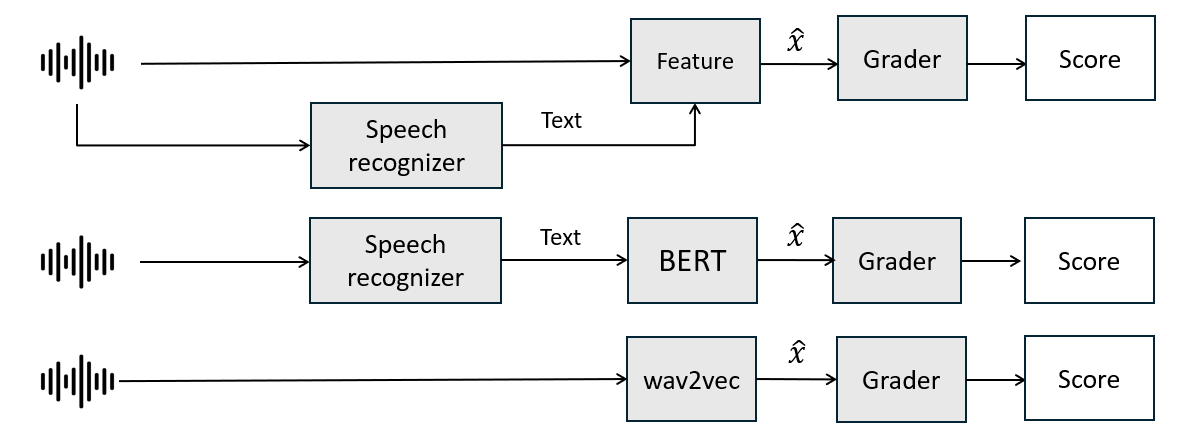
\includegraphics[width=0.7\textwidth]{grader.png}
    \caption{Spoken language assessment system for determining scores under consideration, with feature, text, audio-based model from up to down. ASR: Automatic Speech Recognition}
    \label{fig:grader}
\end{figure}

\nomenclature[Z]{ASR}{Automatic Speech Recognition}

In addition, previous research did not take into account the imbalance of concepts in the dataset, which could affect the CAV performance. Dataset might have more negative concepts than positive concepts. For example, people with their first language (L1) \nomenclature[Z]{L1}{First Language} as Thai is far less than people having other L1. The CAV extraction would not try to weight the minority group higher. Hence, the effect of using balanced weighting in the CAV extraction process is explored. It is shown that despite a difference in CAV extraction, the ability of measuring bias is not affected.

The different types of models differ in terms of the input they take, and the design of the neural network grader. The work therefore attempts to isolate the factors affecting the difference in bias measurement across the models. While the factor affecting the bias sensitivity is yet to be pinpointed, it is found that activation function influences the pattern drastically.

\section{Report Outline}
This report consists of 6 chapters with the following structure:
\begin{itemize}
    \item Chapter \ref{chap:graders} describes the different types of graders which would have its fairness being measured.
    \item Chapter \ref{chap:cav} outlines the steps of CAV extraction.
    \item Chapter \ref{chap:setup} describes the construction of training, calibration and testing data, alongside explanation on model biasing, factor isolation setup, and justification of performance metrics and hyper-parameters.
    \item Chapter \ref{chap:results} presents the results of the experiment, and discusses the implications.
    \item Chapter \ref{chap:conclusions} concludes the report and discusses future work.
\end{itemize}